Long-horizon forecasting is critical in many important applications including risk management and planning. Notable examples include power plant maintenance scheduling \citep{hyndman2009long_electricity} and planning for infrastructure construction~\citep{ziel2018long_epf}, as well as early warning systems that help mitigate vulnerabilities due to extreme weather events~\citep{reid2006early_warning_systems, field2012risk_management_climate}. In healthcare, predictive monitoring of vital signs enables detection of preventable adverse outcomes and application of life-saving interventions~\citep{churpek2016long_healthcare}. 

\begin{figure}[!ht]
    \centering
    \subfigure[\emph{Computational Cost}]{
    \label{fig:computational_cost}
    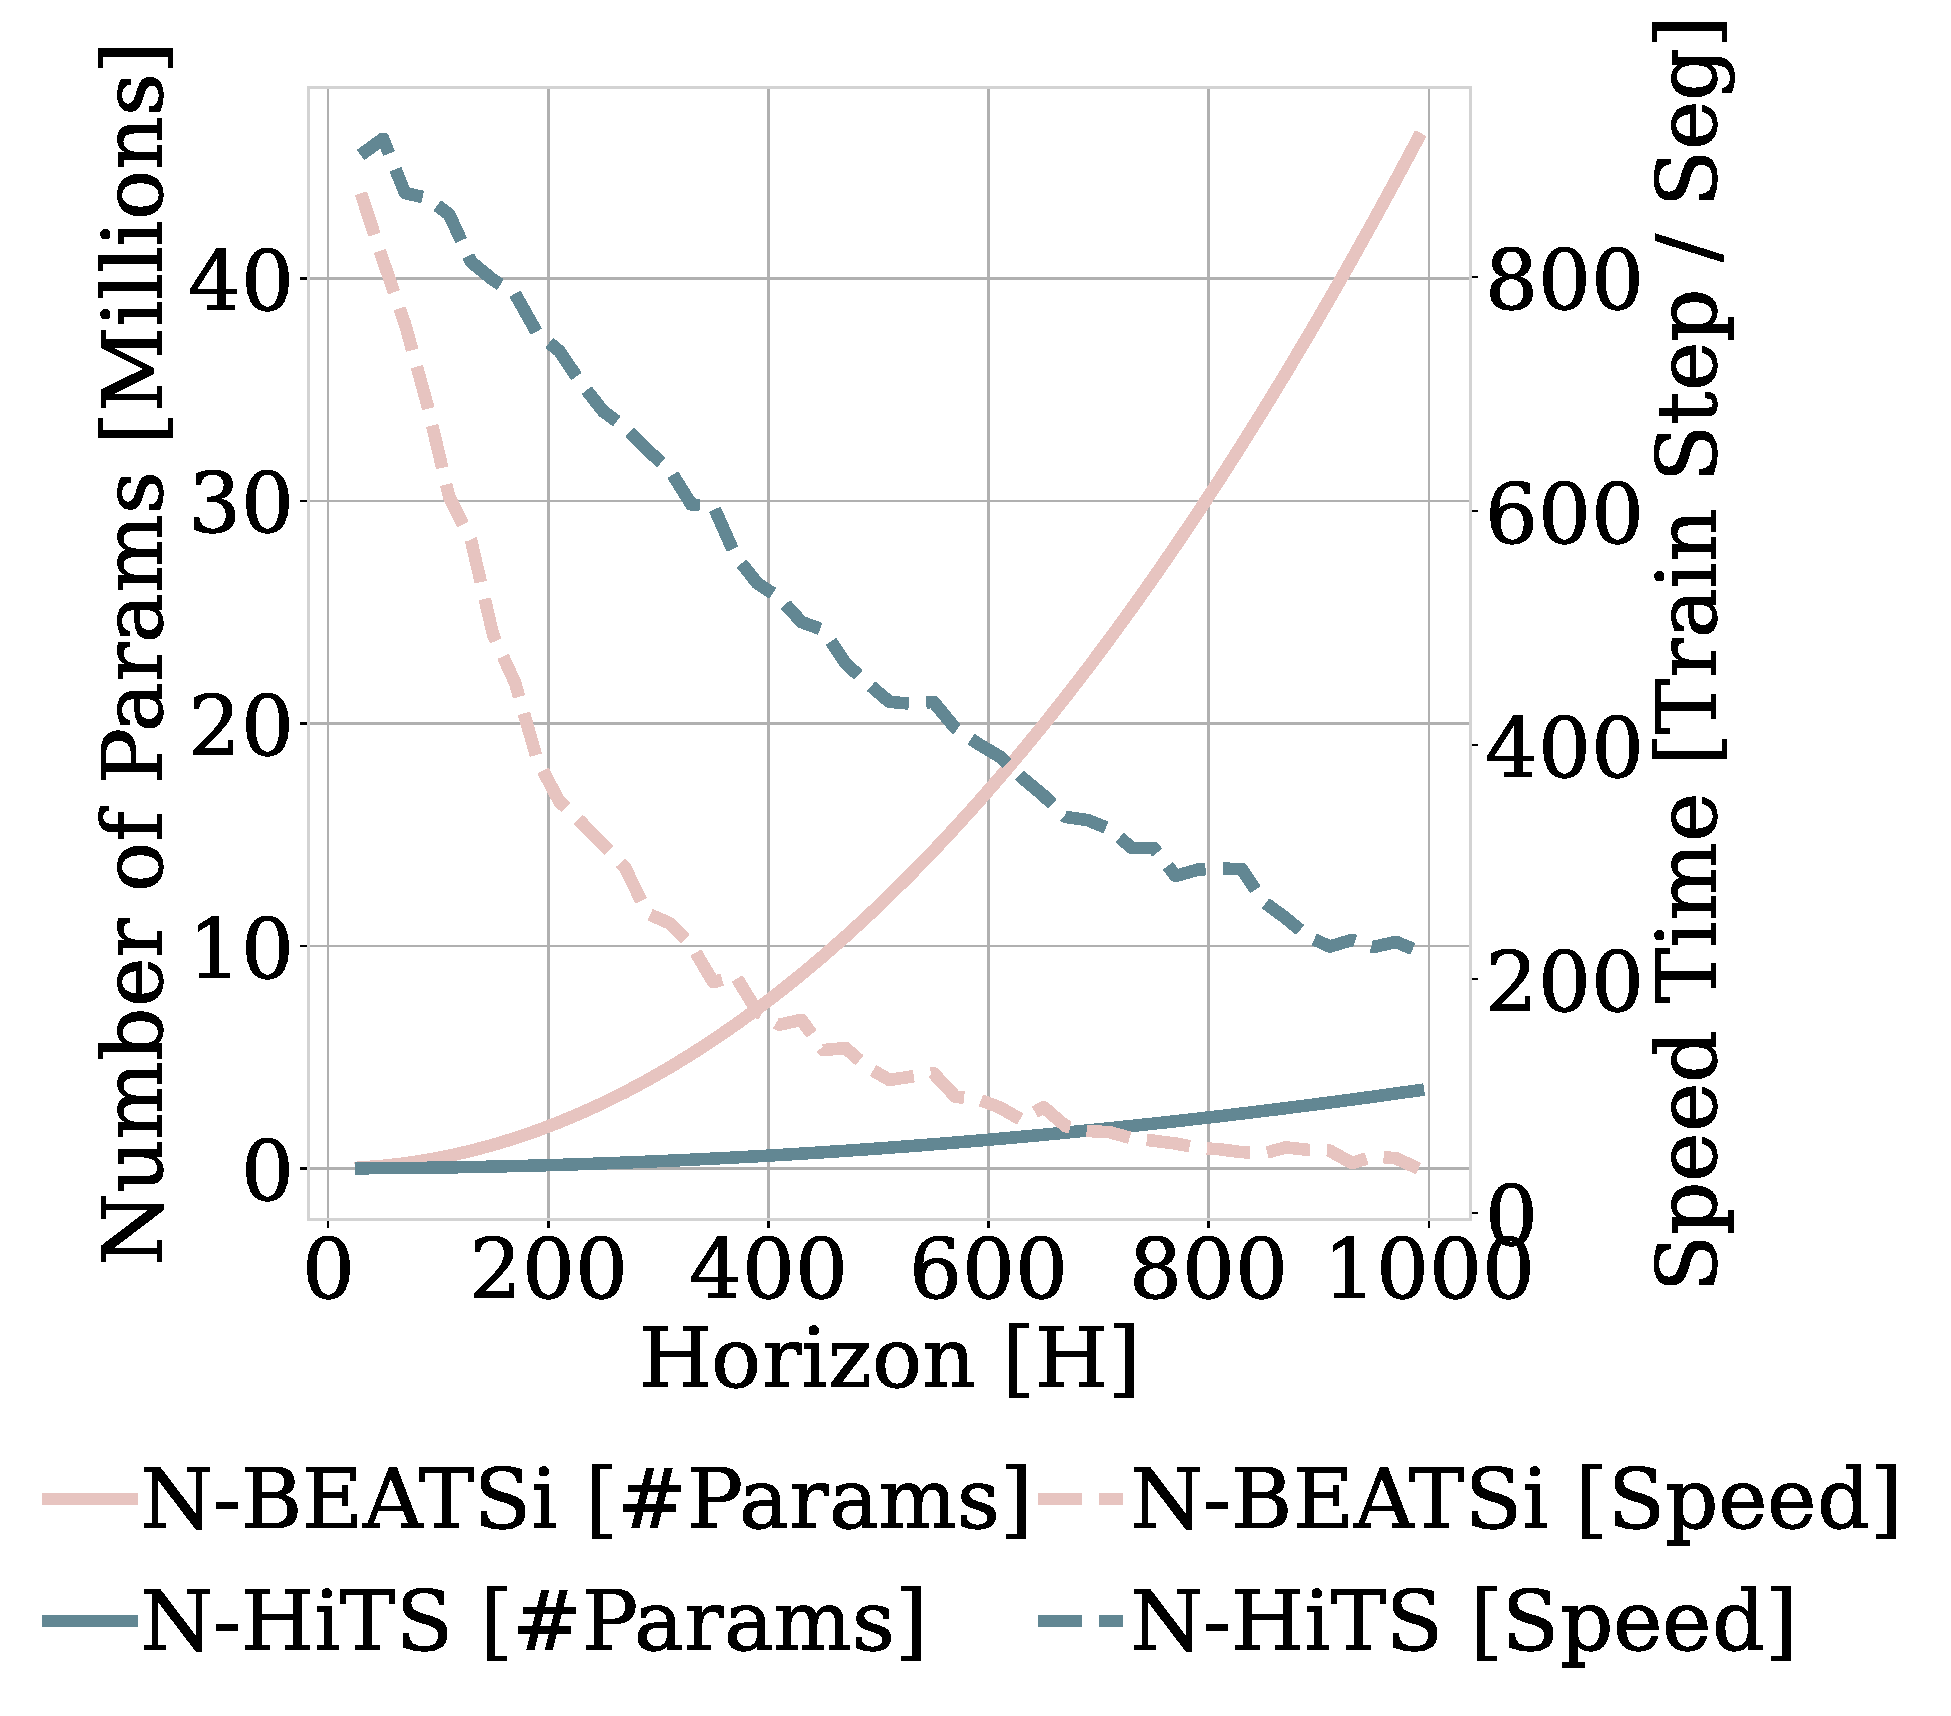
\includegraphics[width=0.46\linewidth]{images/plots-motivation-params-speed.pdf} % 0.51
    }
    \subfigure[\emph{Prediction Errors}]{
    \label{fig:performance}
    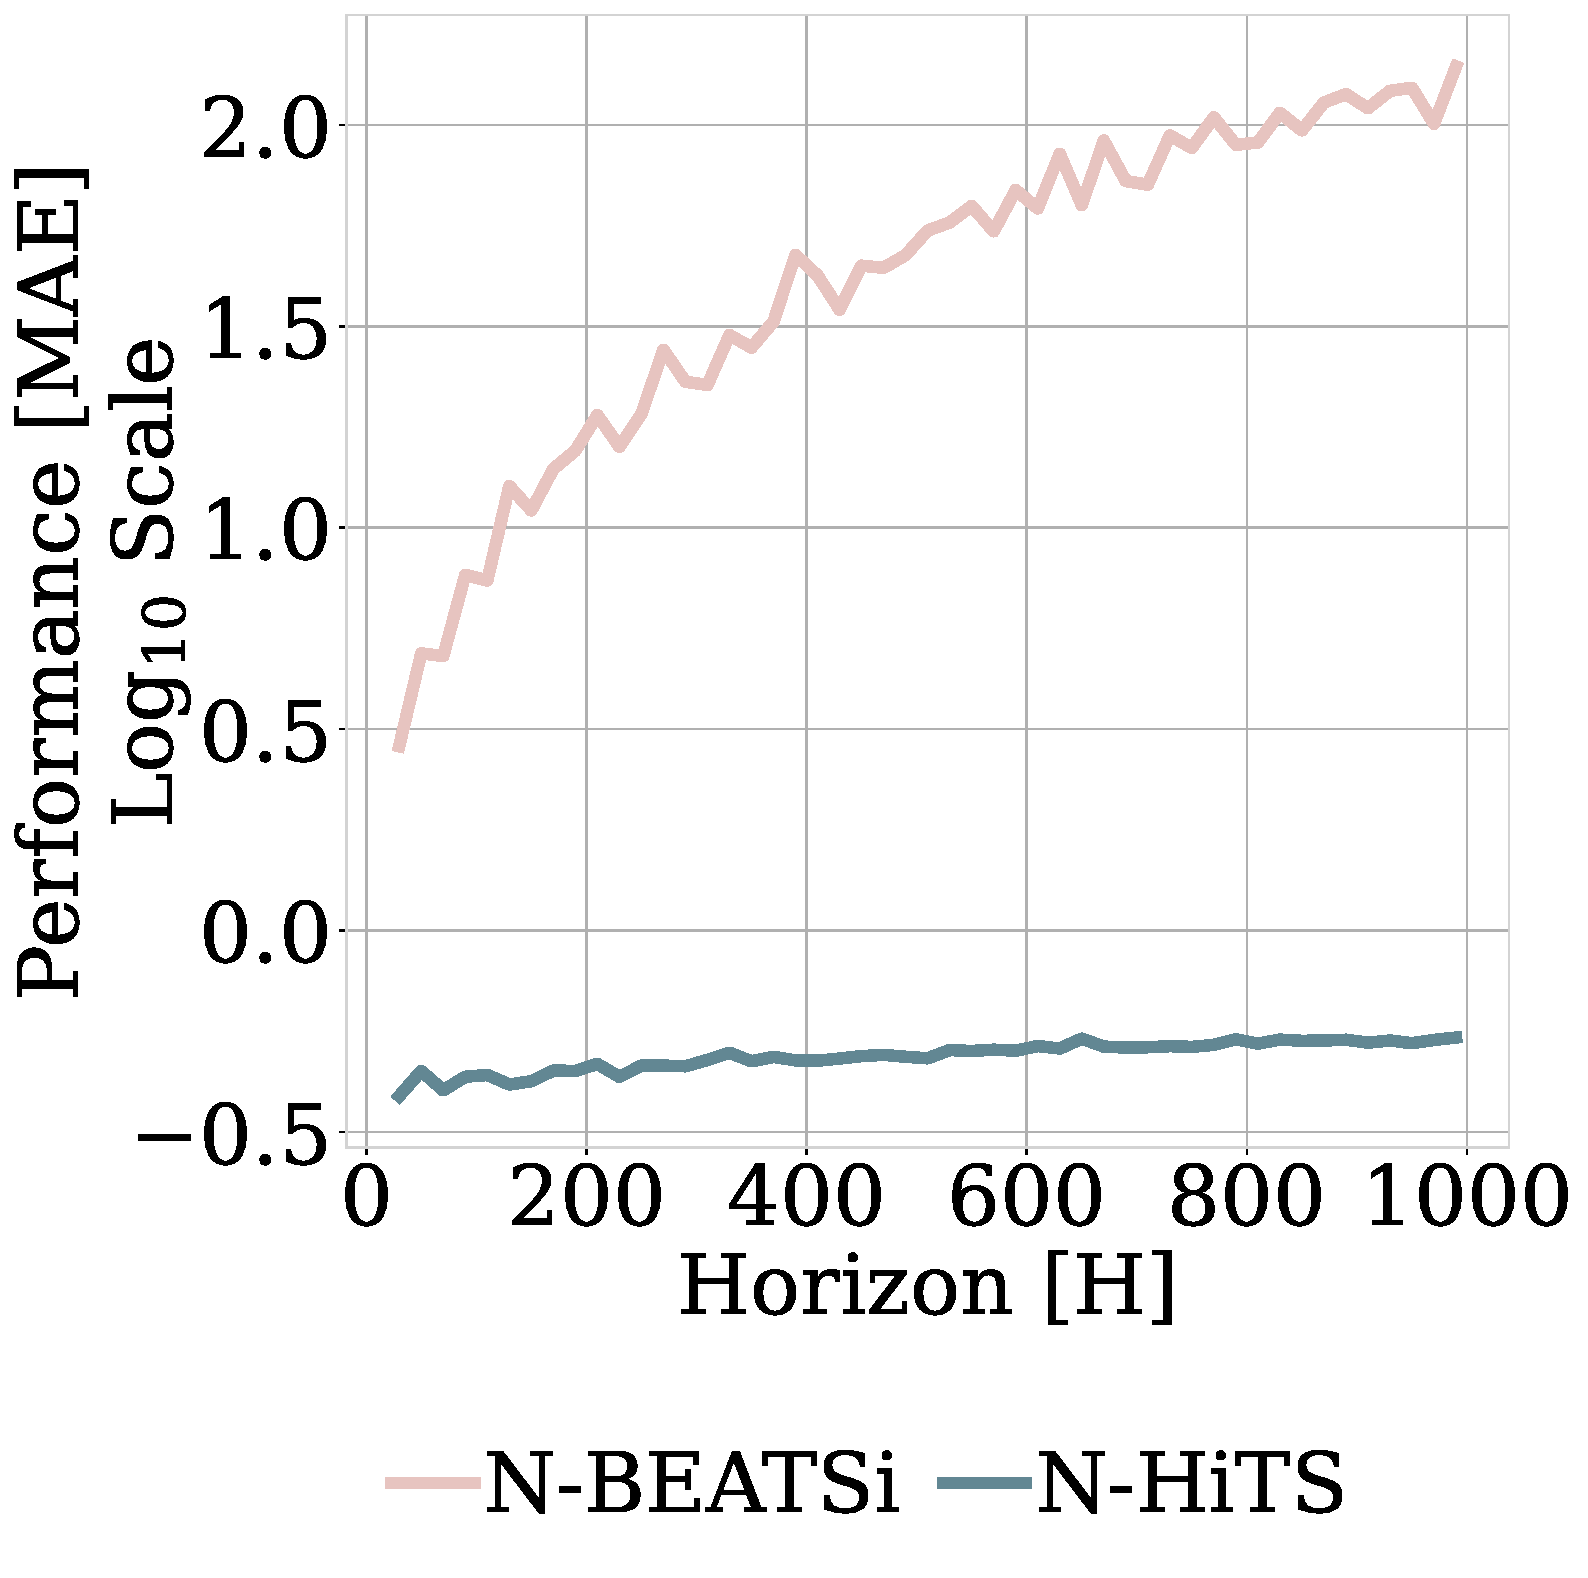
\includegraphics[width=0.40\linewidth]{images/plots-motivation-performance.pdf} % 0.435
    }    
    \subfigure[\emph{Neural Hierarchical Interpolation}]{
    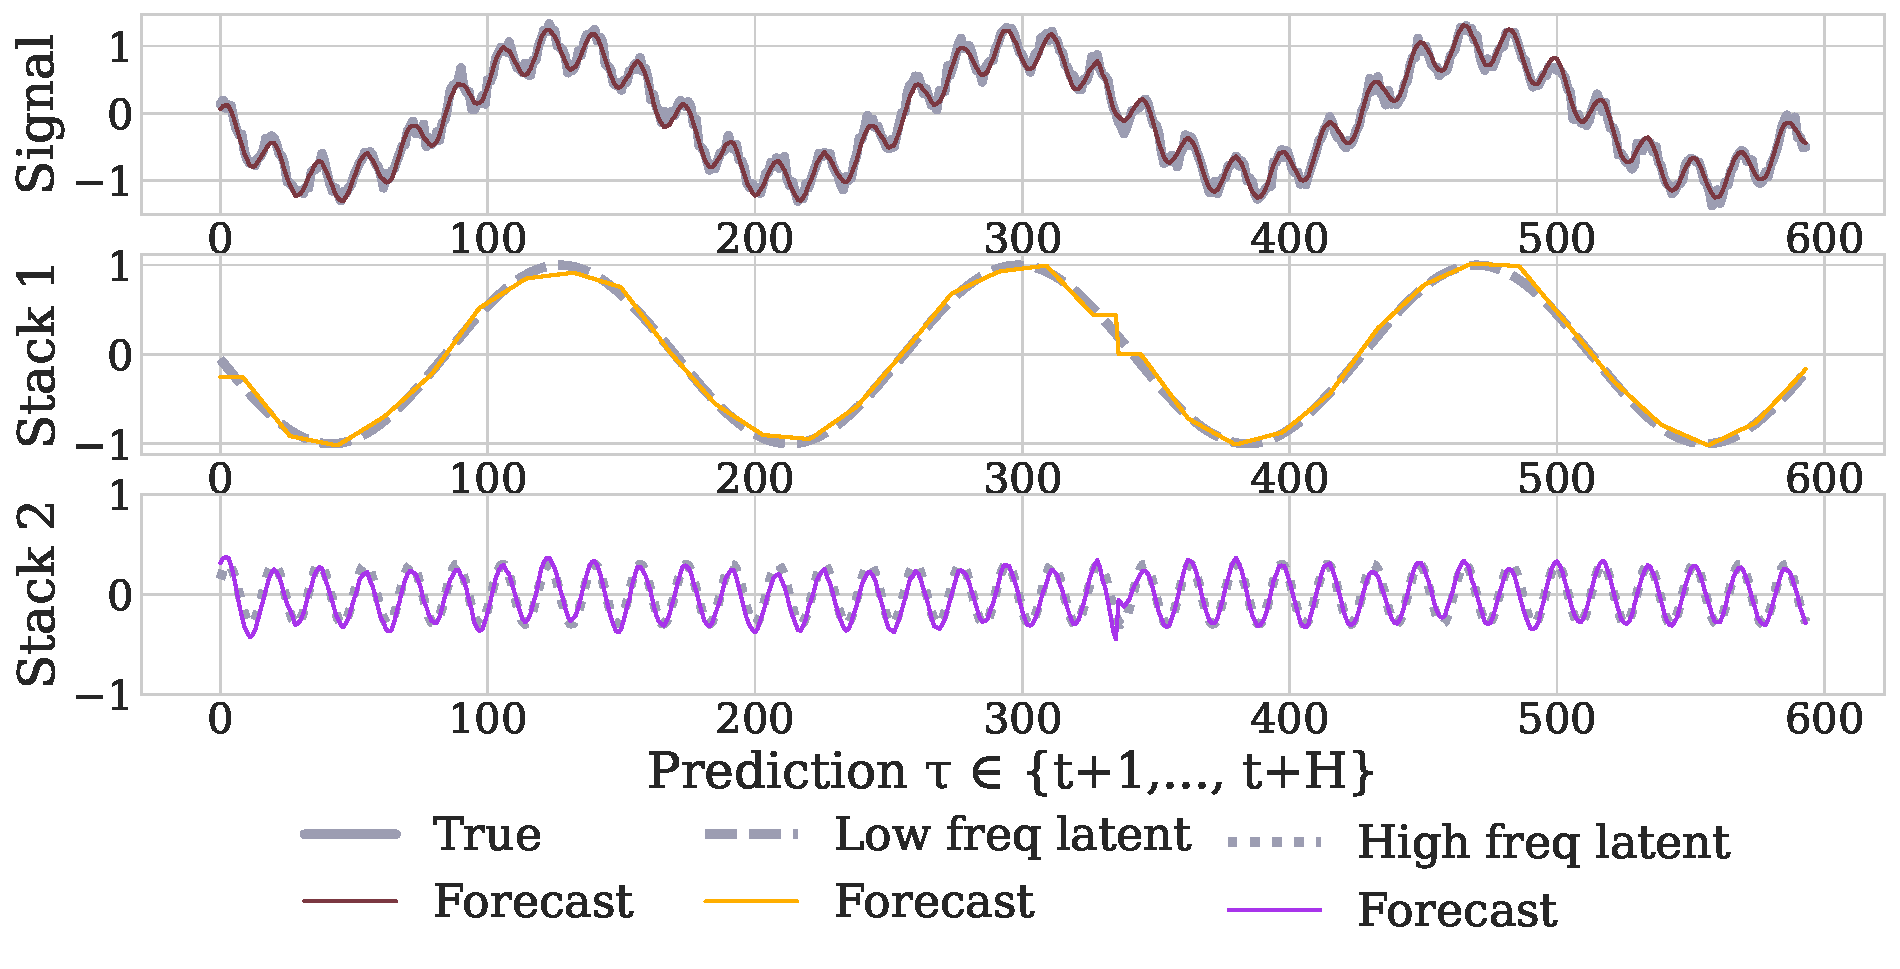
\includegraphics[width=0.85\linewidth]{images/figure1_example_2.pdf} % 0.9
    }
    \caption{(a) The computational costs in time and memory (b) and \emph{mean absolute errors} (MAE) of the predictions of a high capacity fully connected model exhibit evident deterioration with growing forecast horizons. (c) Specializing a flexible model's outputs in the different frequencies of the signal through hierarchical interpolation combined with multi-rate input processing offers a solution.}
    \label{fig:motivation}
\end{figure}

Recently, neural time series forecasting has progressed in a few promising directions. First, the architectural evolution included adoption of the attention mechanism and the rise of Transformer-inspired approaches~\citep{li2019logtrans,fan2019multimodal_transformer,ahmed2019attentive_state_space,lim2021temporal_fusion_transformer}, as well as introduction of attention-free architectures composed of deep stacks of fully connected layers~\citep{oreshkin2020nbeats, olivares2021nbeatsx}. Both of these approaches are relatively easy to scale up in terms of capacity, compared to LSTMs, and have proven to be capable of capturing long-range dependencies. The attention-based approaches are very generic as they can explicitly model direct interactions between every pair of input-output elements. Unsurprisingly, they happen to be the most computationally expensive. The architectures based on fully connected stacks capture input-output relationships implicitly, however they tend to be more compute-efficient. Second, the recurrent forecast generation strategy has been replaced with the multi-step prediction strategy in both of these approaches. Aside from its convenient bias-variance benefits and robustness~\citep{marcellino2006multi_step_forecasting,atiya2016multi_step_forecasting}, the multi-step strategy has enabled the models to efficiently predict long sequences in a single forward pass~\citep{wen2017mqrcnn,zhou2021informer,lim2021temporal_fusion_transformer}.

Despite all the recent progress, long-horizon forecasting remains challenging for neural networks, because their unbounded expressiveness translates directly into \emph{excessive computational complexity} and \emph{forecast volatility}, both of which become especially pronounced in this context. For instance, both attention and fully connected layers scale quadratically in memory and computational cost with respect to the forecasting horizon length. Fig.~\ref{fig:motivation} illustrates how forecasting errors and computation costs inflate dramatically with growing forecasting horizon in the case of the fully connected architecture electricity consumption predictions. Attention-based predictions show similar behavior.

Neural long-horizon forecasting research has mostly focused on attention efficiency making self-attention sparse~\citep{child2019sparse_transformer,li2019logtrans,zhou2021informer} or local~\citep{li2019logtrans}. In the same vain, attention has been cleverly redefined through locality-sensitive hashing~\citep{kitaev2020reformer} or FFT~\citep{wu2021autoformer}. Although that research has led to incremental improvements in compute cost and accuracy, the silver bullet long-horizon forecasting solution is yet to be found. In this paper we make a bold step in this direction by developing a novel forecasting approach that cuts long-horizon compute cost by an order of magnitude while simultaneously offering \multivarMSEgains\% accuracy improvements on a large array of multi-variate forecasting datasets compared to existing state-of-the-art Transformer-based techniques. We redefine existing fully-connected \NBEATS{} architecture~\citep{oreshkin2020nbeats} by enhancing its input decomposition via multi-rate data sampling and its output synthesizer via multi-scale interpolation. Our extensive experiments show the importance of the proposed novel architectural components and validate significant improvements in accuracy and computational complexity of the proposed algorithm. \\

Our contributions are summarized below:
\begin{enumerate}%[label=(\roman*)]
    \item \textbf{Multi-Rate Data Sampling}: We incorporate sub-sampling layers in front of fully-connected blocks, significantly reducing the memory footprint and the amount of computation needed, while maintaining the ability to model long-range dependencies. 
    \item \textbf{Hierarchical Interpolation}: We enforce smoothness of the multi-step predictions by reducing the dimensionality of neural network's prediction and matching its time scale with that of the final output via multi-scale hierarchical interpolation. This novel technique is not unique to our proposed model, and can be incorporated in different architectures.
    \item \textbf{\ourstext \ architecture}: A novel way of hierarchically synchronizing the rate of input sampling with the scale of output interpolation across blocks, which induces each block to specialize on forecasting its own frequency band of the time-series signal.
    \item \textbf{State-of-the-art results} on six large-scale benchmark datasets from the long-horizon forecasting literature: electricity transformer temperature, exchange rate, electricity consumption, San Francisco bay area highway traffic, weather and influenza-like illness. % on six well-established multivariate forecasting benchmarks.
\end{enumerate}

%Our code is available at
%\url{https://anonymous.4open.science/r/n-hits-C430}
% \href{https://github.com/cchallu/deep-midas}{\textcolor{blue}{\ours's repository}}.

The remainder of this paper is structured as follows. Section~\ref{section2:literature} reviews relevant literature, Section~\ref{section3:model} introduces notation and describes the methodology, Sections~\ref{section4:experiments} and~\ref{section:discussion_of_findings} describe and analyze our empirical findings. Finally, Section \ref{section5:conclusion} concludes the paper.
